\documentclass{article}
\usepackage{graphicx}
\usepackage{float}
\usepackage{amsmath}
\graphicspath{{images/}}
\usepackage{caption}
\captionsetup[figure]{position = below,}
\usepackage{listings}
\usepackage{xcolor}
\usepackage{amssymb}
 \usepackage{amsthm}
 \usepackage{amsfonts}
\usepackage{braket}
\DeclareCaptionFont{white}{\color{white}}
\DeclareCaptionFormat{listing}{%
\parbox{\textwidth}{\colorbox{gray}{\parbox{\textwidth}{#1#2#3}}\vskip-4pt}}
\captionsetup[lstlisting]{format=listing,labelfont=white,textfont=white}
\lstset{frame=lrb,xleftmargin=\fboxsep,xrightmargin=-\fboxsep, columns=fullflexible}


\title{\textbf{Grover's Search Algorithm}}

\author{Indranil Ghosh\\Jadavpur University, Physics Department\\ UG-III\\ Email: indranilg49@gmail.com}

\date{\today}

\begin{document}
\maketitle

\begin{abstract}
This project is to compare the simulation of Grover's search algorithm for two qubit systems, between IBM's Quantum Experience's real quantum simulator and a  Python program that  has been designed, available in Github (https://github.com/indrag49/Quantum-SimuPy), for  simulating the ideal case. Packages used: Numpy, Pandas and Mathplotlib. The quantum gates and the functions required for this simulation are available in the program and can be easily implemented. The moto of this project is to use python packages to design a quantum simulator for performing simple quantum computations.
\end{abstract}

\section{Introduction}
Grover's Algorithm, devised by \textit{Lov Grover} in the year 1996, is a quantum search algorithm, that searches through a N-dimensional search space. Instead of searching for the desired element, the algorithm focuses its search on the index of the element, $i$, such that $i \in[0, N)$. The \textit{amplitude amplification trick} is used as a core process here and the algorithm takes $\mathcal{O}$($\sqrt{N}$) steps to achieve its goal compared to  $\mathcal{O}$(N) steps taken by the classical counterpart.

\section{The Problem}
Suppose there is a database with $N$ unsorted elements. We want to locate the index an element with a desired property, marked \textit{\textbf{w}} from this database. We assume the value of N in such a way that the index can be stored in $n=\log_2{N}$ bits, i.e., $N=2^n$. This search problem has M solutions such that $1<=M<=N$. For a classical search, $M={N \over 2}$ on average and $M=N$ for the worst case scenario. But, on a quantum computer, $M$ is roughly $\sqrt{N}$. Thse Grover's search algorithm provides a quadratic speedup, which is  a time-saver for long lists, i.e for problems which may take million of years for the most powerful classical supercomputers in our possession, to solve.

\section{What Is The Oracle?}
The convinient way to encode the given list of $N$ terms is by a function $f$ such that $f(x)=\delta_{xw}$ where $(x, w) \in [0, N-1]$. 
\begin{center}
$f(x)=1, x=w$\\ \par
$f(x)=0, x \ne w$
\end{center}
It follows $f(w)=1$ for the winning index. At first we choose a binary encoding of the system , $x, w \in [0, 1]^n$ and represent the indices in terms of qubits in a quantum computer($x$ maps to $0$ and $w$ maps to $1$). Next we define the \textit{Oracle}, a quantum black box, $U_f$ which is itself a unitary matrix, such that,
\begin{center}
$U_f \ket{x}=- \ket{x}$ for $x=w, f(x)=1$, x is a solution of the search\\ \par
$U_f \ket{x}= \ket{x}$ for $x \ne w, f(x)=0$, x is not a solution of the search
\end{center}
It is established that $U_f \ket{x}=(-1)^{f(x)} \ket{x}$. \\ \par
The action of the \textit{Oracle} can also be depicted as, 
\begin{center}
$U_f \ket{x} \ket{q} = \ket{x} \ket{q \bigoplus f(x)}$
\end{center}
Here, $\ket{x}$ is the index register, $\bigoplus$ denotes addition modulo $2$ and the oracle qubit $\ket{q}$, a single qubit which flips if $f(x)=1$ and else remains unchanged. It is seen that with $N$ items with $M$ solutions we need to apply the search oracle $\mathcal{O}(\sqrt{N \over M})$ times to attain the solution.

\section{A Deep Dive Into The Amplitude Amplification Technique}
The algorithm uses single $n$ qubit register and its goal is to find the solution of the search by applying the smallest number of oracles possible. In the beginning, the computer is in the state $\ket{0}^{\bigoplus n}$. Application of the Hadamard transform puts the computer in the state of uniform superposition $\ket{s}$,
\begin{center}
$\ket{s} = {1 \over \sqrt{N}} \sum_{x=0}^{x=N-1} \ket{x}$
\end{center}
Now, performing a measurement in the standard basis would result in the collapse of the superposition to any one of the basis states with the same probability of $2^{-n}$. Hence, we need to try about $2^n$ steps on average to guess the correct result. The application of the Amplitude Amplification enhances the probability of the winning state to be located by the quantum computer. We consider two special states: the superposition state $\ket{s}$ and the winning state $\ket{w}$.\par
For the winning state, the oracle, $U_f$=$U_w$=$I-2 \ket{w} \bra{w}$. We prove this from the following computations :
\begin{center}
$(I-2 \ket{w} \bra{w}) \ket{w}=\ket{w}-2\ket{w}\braket{w|w}=\ket{w}-2\ket{w}=-\ket{w}={U_w}\ket{w}$, for $x=w$ \par
$(I-2 \ket{w} \bra{w}) \ket{x}=\ket{x}-2\ket{w}\braket{w|x}=\ket{x}-0=\ket{x}={U_w}\ket{x}$, for $x \ne w$
\end{center}
Now, we note the following computations:
\begin{center}
1. $\braket{w|s}={1 \over \sqrt{N}}\sum_{x=0}^{N-1} \braket{w|x}={1 \over \sqrt{N}}=\braket{s|w}$ \par
2. $\braket{s|s}={1 \over \sqrt{N}} {1 \over \sqrt{N}}\sum_{x=0}^{N-1}\sum_{x=0}^{N-1} \braket{x|x}={1 \over N}N=1$
\end{center}
Besides the oracle, we also need another reflection operator, Grover's Diffusion operator, $U_s=2\ket{s}\bra{s}-I$.
\section{Algorithm Procedure}
\begin{figure}[H]
\centering 
\noindent\makebox[\textwidth]{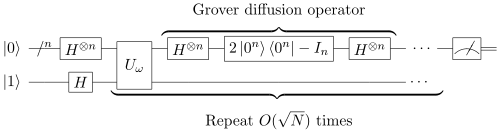
\includegraphics[scale=0.6]{Grover}}%
\caption{Grover's Algorithm Circuit [Figure from Wikipedia]}
\end{figure}
We now state the Grover's iterator.After preparation of the superposition state we apply the oracle reflection $U_w$ to the state, which corresponds the reflection of the state to $-\ket{w}$.
\begin{center}
$U_w \ket{s} = (I-2\ket{w} \bra{w})\ket{s}$\par
$=I\ket{s}-2\ket{w}\braket{w|s}$\par
$=\ket{s}-{2\over{\sqrt{N}}}\ket{w}$
\end{center}
This transformation means that the amplitude in front of the winning state becomes negative and the average amplitude decreases.\par
Now the additional reflection $U_s$ is applied to the resultant state, $\ket{s}-{2\over{\sqrt{N}}}\ket{w}$. We see, Grover's diffusion Operator, $U_s=H^{\otimes n}(2\ket{0^n}\bra{0^n}-I)H^{\otimes n}=2(H^{\otimes n}\ket{0^n}\bra{0^n}H^{\otimes n})-H^{\otimes n}H^{\otimes n}=2\ket{s}\bra{s}-I$, as stated above. Now,
\begin{center}
$U_s(\ket{s}-{2\over{\sqrt{N}}}\ket{w})=(2\ket{s}\bra{s} - I)(\ket{s}-{2\over{\sqrt{N}}}\ket{w})$\par
$=2\ket{s}\braket{s|s}-\ket{s}-{4\over \sqrt{N}}\ket{s}\braket{s|w}+{2\over \sqrt{N}}\ket{w}$\par
$=2\ket{s}-\ket{s}-{4\over \sqrt{N}}{1\over \sqrt{N}}\ket{s}+{2\over \sqrt{N}}\ket{w}$\par
$=\ket{s}-{4\over \sqrt{N}}\ket{s}+{2\over \sqrt{N}}\ket{w}$\par
$={{N-4}\over N}\ket{s}+{2\over \sqrt{N}}\ket{w}$
\end{center}
This two reflections corresponds to a rotation, that is rotates the initial state $\ket{s}$ towards the winner $\ket{w}$. Since the average amplitude was lowered by the first reflection, the second transformation boosts the negative amplitude of $\ket{w}$ to rougly three times its original value and lowers the other amplitudes.\par
We see that we need to apply the Grover's iterator roughly $\sqrt{N}$ times to concentrate on the winner. We note that in our simulations, we have considered $n=2$, i.e $N=4$. So ${{N-4}\over N}\ket{s}+{2\over \sqrt{N}}\ket{w}=\ket{w}$ for$N=4$. The single application of the Grover's iterator returns us the winner index.
\section{Comparisons for Circuits for $n=2$, i.e, $N=4$}
As $N=4$, there are 4 possible oracles $U_f$, one for each choice of the winner. The first part of the examples creates the superposition state $\ket{s}$, the second part applies the oracle $U_f$ on $\ket{s}$ and the last part applies $U_s$ on $U_f \ket{s}$.
\subsection{A=00}
\subsubsection{IBM Quantum Experience results}
\begin{figure}[H]
\centering 
\noindent\makebox[\textwidth]{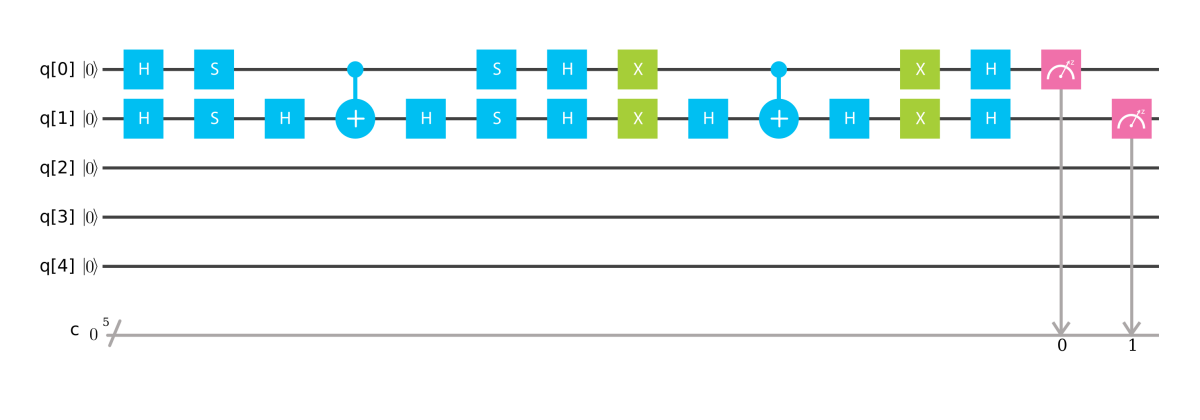
\includegraphics[scale=0.3]{A00}}%
\caption{Algorithm Circuit[Figure from IBM Q experience's home page]}
\end{figure}
\begin{figure}[H]
\centering 
\noindent\makebox[\textwidth]{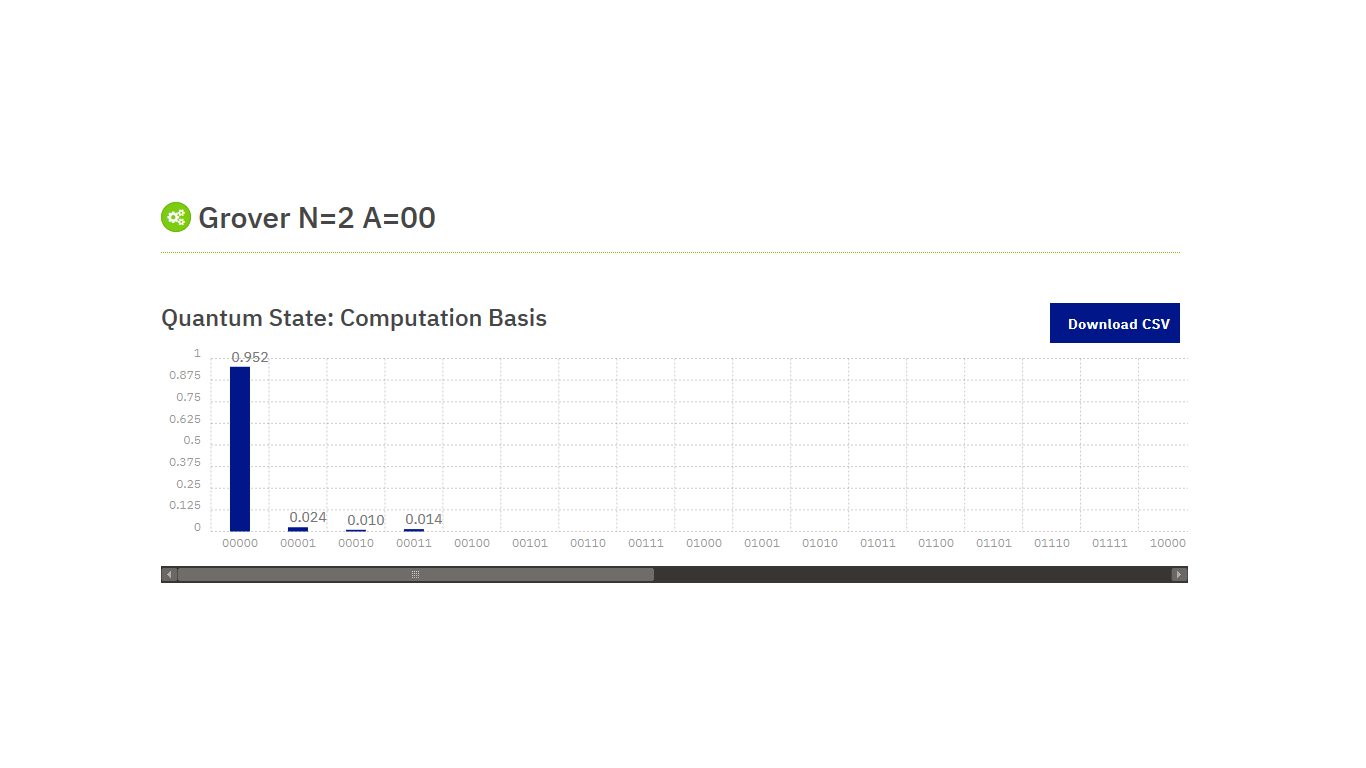
\includegraphics[scale=0.3]{A00_result}}%
\caption{Probability Distribution, with noise[Figure from IBM Q experience's home page]}
\end{figure}
\subsubsection{Python Simulation}
\begin{lstlisting}[frame=single, language=Python]
k=np.kron
H=Hadamard(I2)
H_n=k(H, H)
h=k(I2, H)
# Uf
s=k(Phase(I2), Phase(I2))
s=h.dot(s)
s=CNOT(s)
s=h.dot(s)
Uf=k(Phase(I2), Phase(I2)).dot(s)
# Us
X_n=k(PauliX(I2), PauliX(I2))
t=h.dot(X_n.dot(H_n))
u=CNOT(t)
g=H_n.dot(X_n.dot(h))
Us=g.dot(u)
Gate=Us.dot(Uf.dot(H_n))
m=measure(Gate.dot(Q00))
print(m)
plot_measure(m)
\end{lstlisting}
\begin{figure}[H]
\centering 
\noindent\makebox[\textwidth]{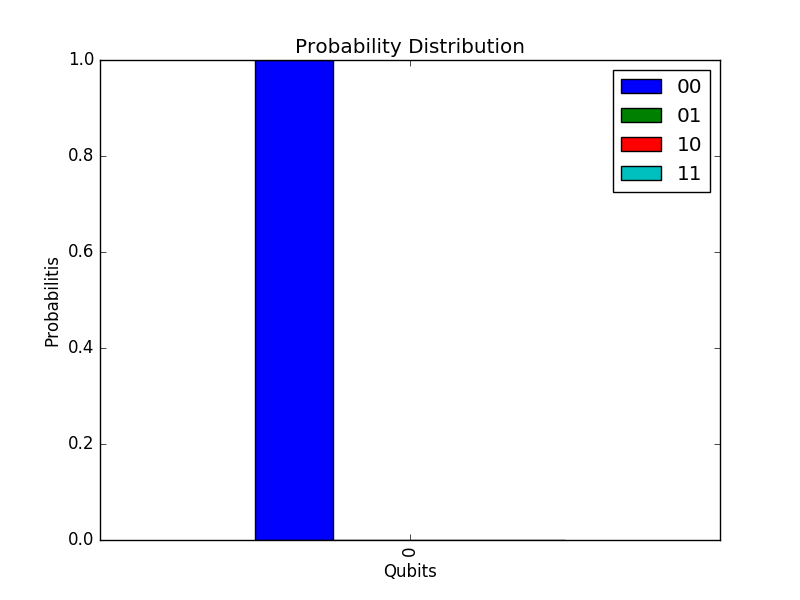
\includegraphics[scale=0.3]{A00_1}}%
\caption{Probability Distribution, without noise}
\end{figure}
\subsection{A=01}
\subsubsection{IBM Quantum Experience results}
\begin{figure}[H]
\centering 
\noindent\makebox[\textwidth]{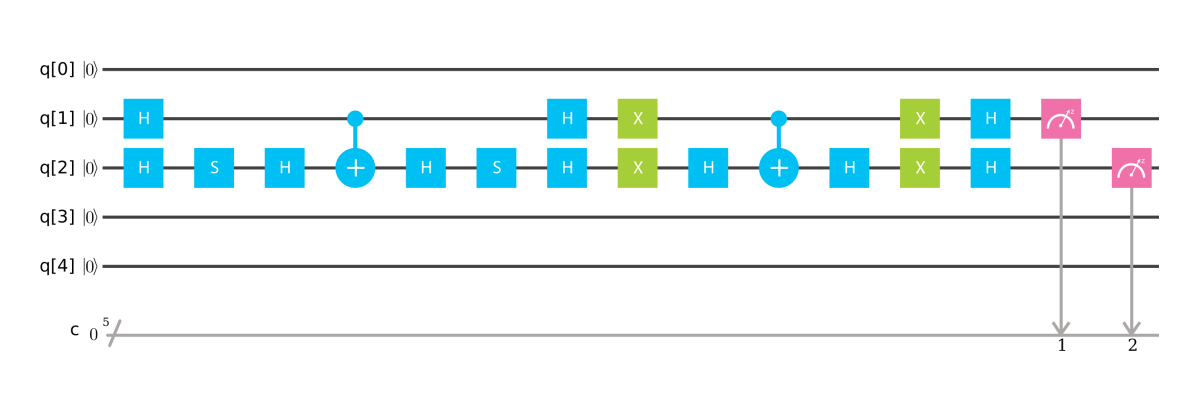
\includegraphics[scale=0.3]{A01}}%
\caption{Algorithm Circuit[Figure from IBM Q experience's home page]}
\end{figure}
\begin{figure}[H]
\centering 
\noindent\makebox[\textwidth]{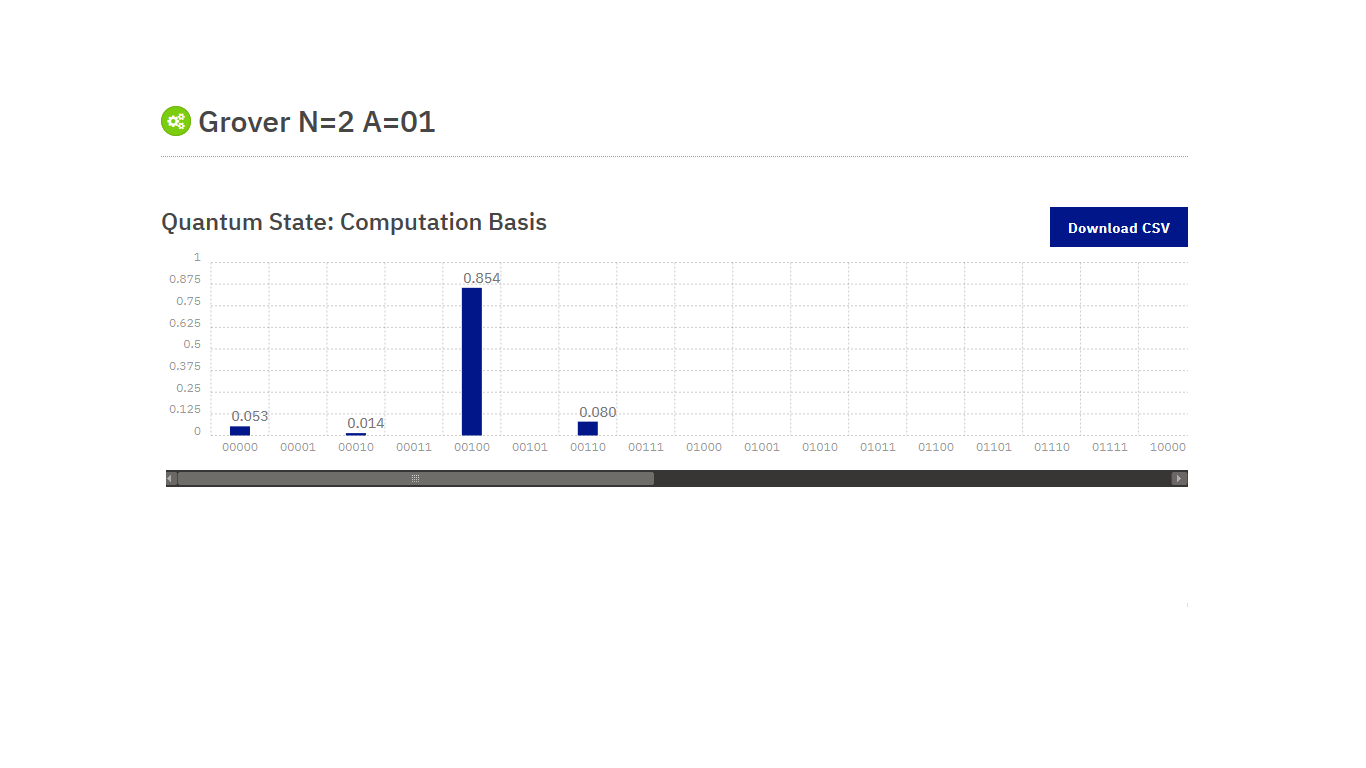
\includegraphics[scale=0.3]{A01_result}}%
\caption{Probability Distribution, with noise[Figure from IBM Q experience's home page]}
\end{figure}
\subsubsection{Python Simulation}
\begin{lstlisting}[frame=single, language=Python]
k=np.kron
H=Hadamard(I2)
H_n=k(H, H)
h=k(I2, H)
# Uf
s=k(I2, Phase(I2))
s=h.dot(s)
s=CNOT(s)
s=h.dot(s)
Uf=k(I2, Phase(I2)).dot(s)
# Us
X_n=k(PauliX(I2), PauliX(I2))
t=h.dot(X_n.dot(H_n))
u=CNOT(t)
g=H_n.dot(X_n.dot(h))
Us=g.dot(u)
Gate=Us.dot(Uf.dot(H_n))
m=measure(Gate.dot(Q00))
print(m)
plot_measure(m)
\end{lstlisting}
\begin{figure}[H]
\centering 
\noindent\makebox[\textwidth]{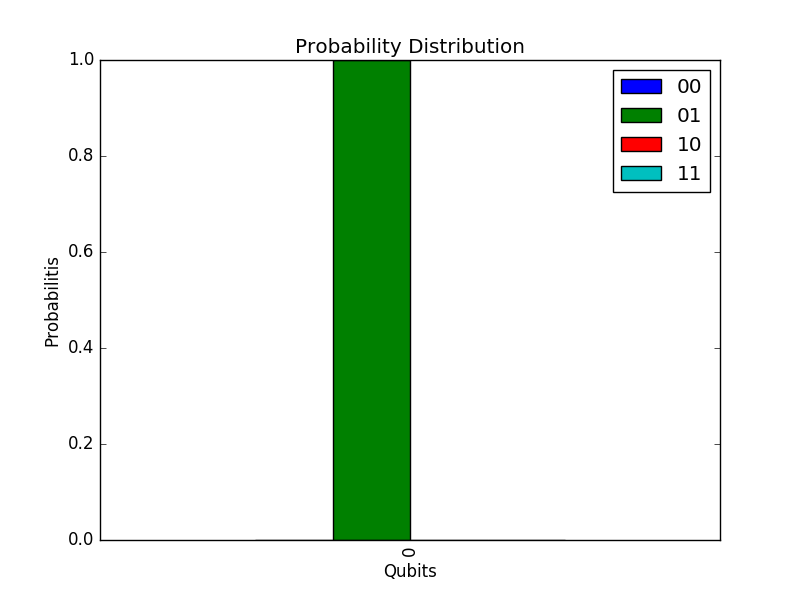
\includegraphics[scale=0.3]{A01_1}}%
\caption{Probability Distribution, without noise}
\end{figure}
\subsection{A=10}
\subsubsection{IBM Quantum Experience results}
\begin{figure}[H]
\centering 
\noindent\makebox[\textwidth]{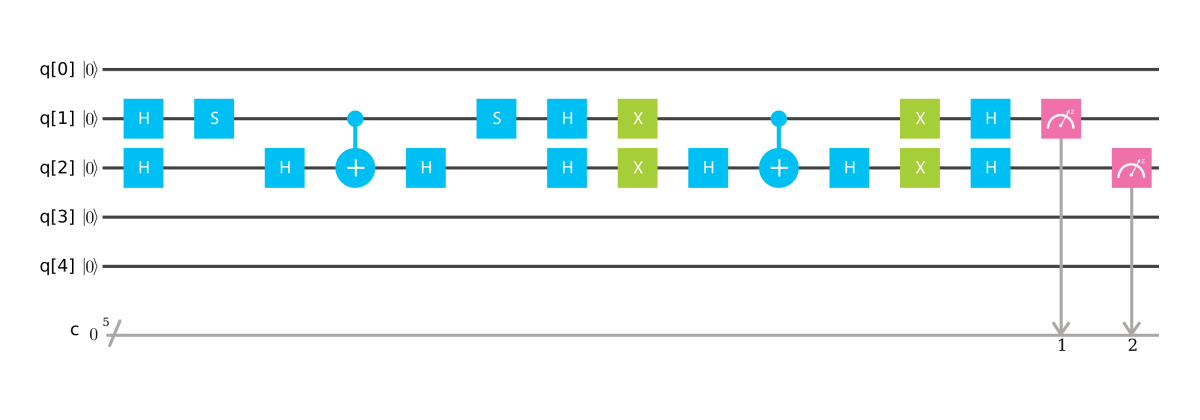
\includegraphics[scale=0.3]{A10}}%
\caption{Algorithm Circuit[Figure from IBM Q experience's home page]}
\end{figure}
\begin{figure}[H]
\centering 
\noindent\makebox[\textwidth]{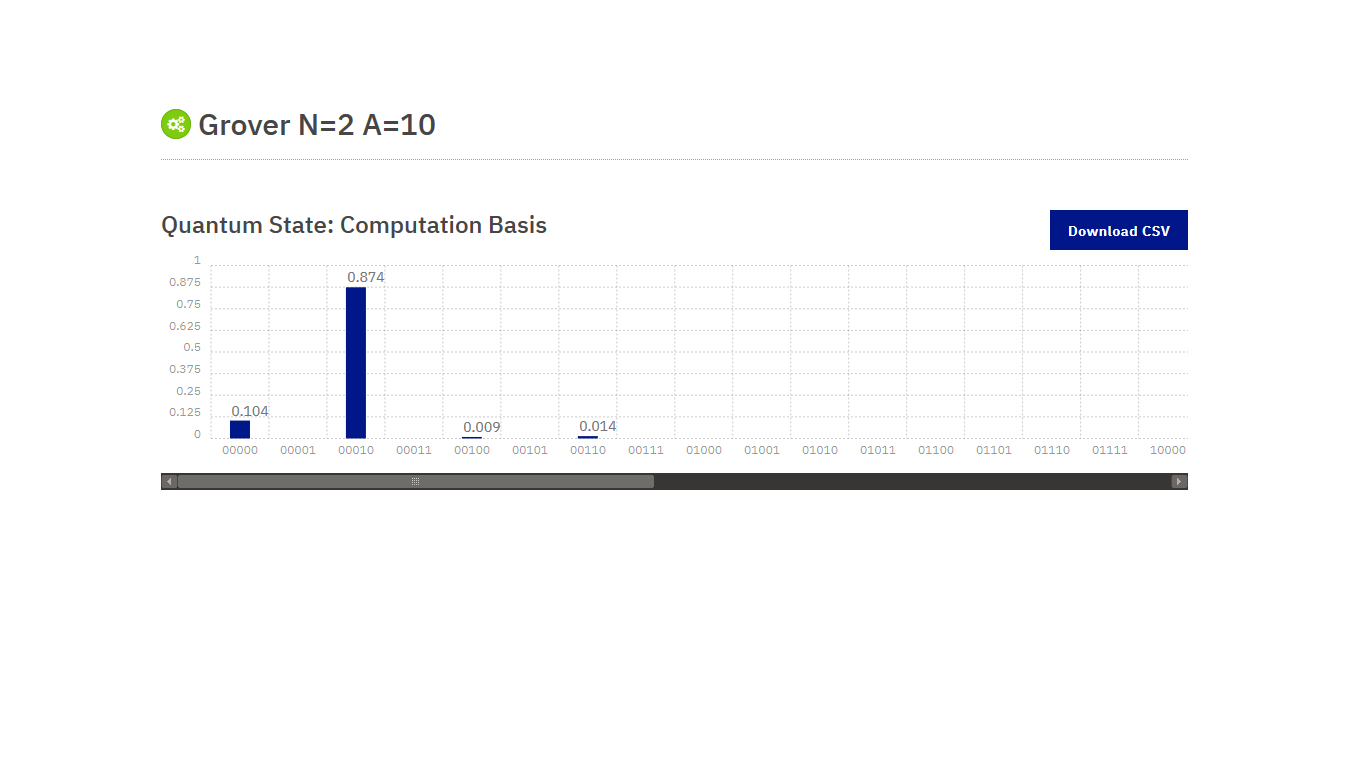
\includegraphics[scale=0.3]{A10_result}}%
\caption{Probability Distribution, with noise[Figure from IBM Q experience's home page]}
\end{figure}
\subsubsection{Python Simulation}
\begin{lstlisting}[frame=single, language=Python]
k=np.kron
H=Hadamard(I2)
H_n=k(H, H)
h=k(I2, H)
# Uf
s=k(Phase(I2), I2)
s=h.dot(s)
s=CNOT(s)
s=h.dot(s)
Uf=k(Phase(I2), I2).dot(s)
# Us
X_n=k(PauliX(I2), PauliX(I2))
t=h.dot(X_n.dot(H_n))
u=CNOT(t)
g=H_n.dot(X_n.dot(h))
Us=g.dot(u)
G=Us.dot(Uf)
Gate=Us.dot(Uf.dot(H_n))
m=measure(Gate.dot(Q00))
print(m)
plot_measure(m)
\end{lstlisting}
\begin{figure}[H]
\centering 
\noindent\makebox[\textwidth]{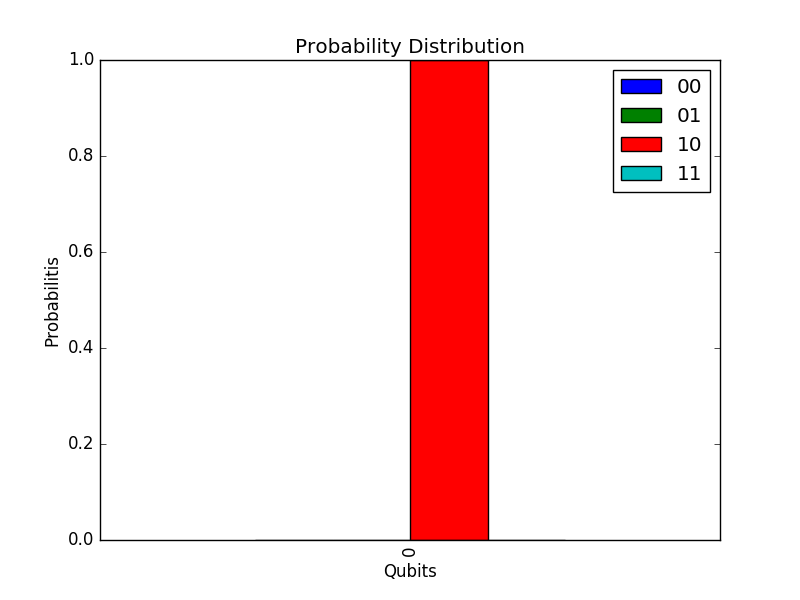
\includegraphics[scale=0.3]{A10_1}}%
\caption{Probability Distribution, without noise}
\end{figure}
\subsection{A=11}
\subsubsection{IBM Quantum Experience results}
\begin{figure}[H]
\centering 
\noindent\makebox[\textwidth]{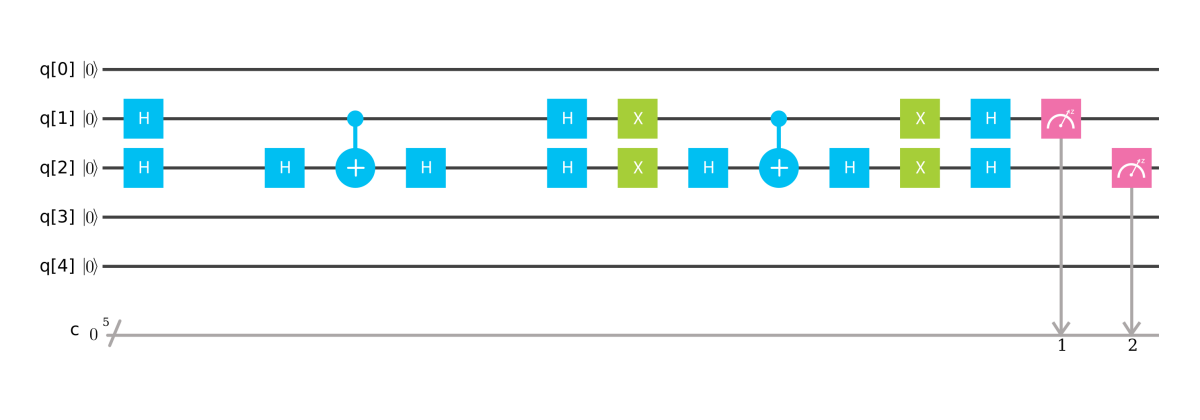
\includegraphics[scale=0.3]{A11}}%
\caption{Algorithm Circuit[Figure from IBM Q experience's home page]}
\end{figure}
\begin{figure}[H]
\centering 
\noindent\makebox[\textwidth]{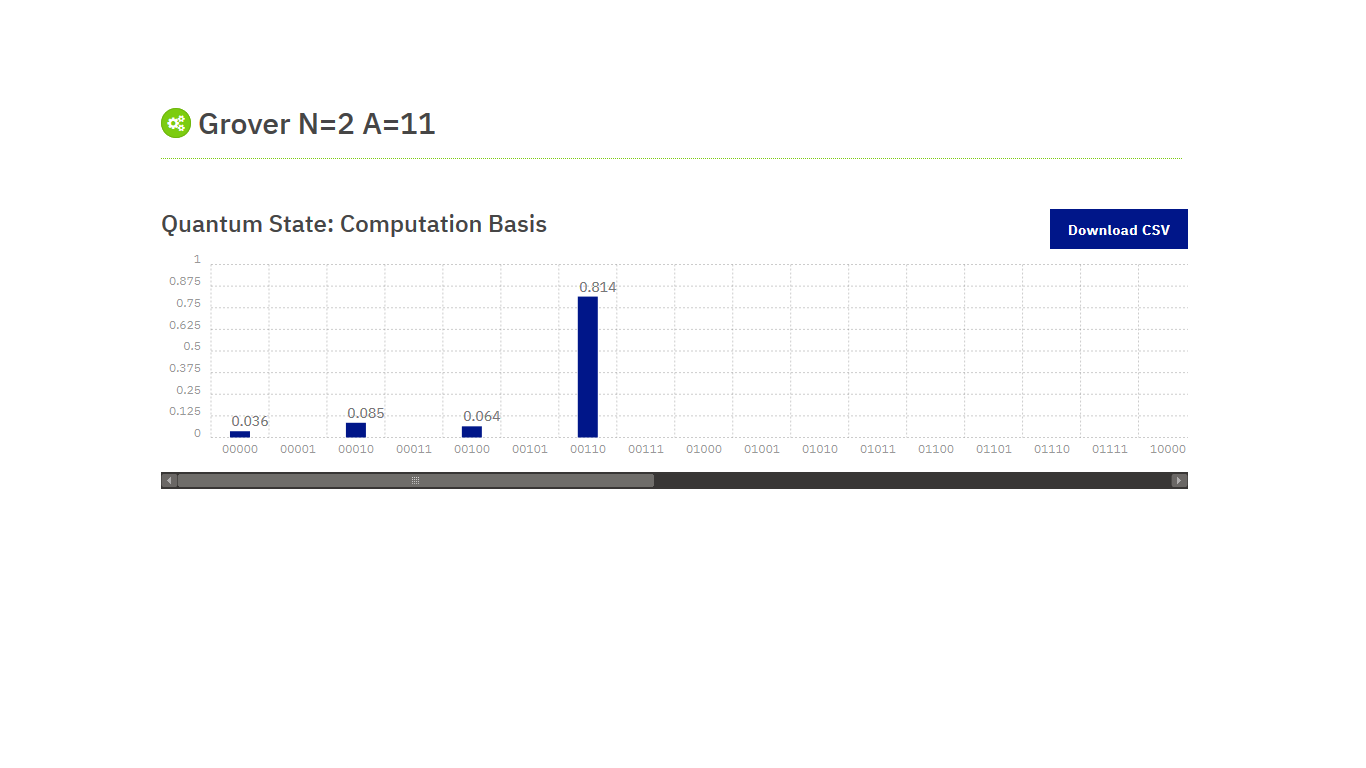
\includegraphics[scale=0.3]{A11_result}}%
\caption{Probability Distribution, with noise[Figure from IBM Q experience's home page]}
\end{figure}
\subsubsection{Python Simulation}
\begin{lstlisting}[frame=single, language=Python]
k=np.kron
H=Hadamard(I2)
H_n=k(H, H)
h=k(I2, H)
# Uf
s=k(I2, I2)
s=h.dot(s)
s=CNOT(s)
s=h.dot(s)
Uf=k(I2, I2).dot(s)
# Us
X_n=k(PauliX(I2), PauliX(I2))
t=h.dot(X_n.dot(H_n))
u=CNOT(t)
g=H_n.dot(X_n.dot(h))
Us=g.dot(u)
G=Us.dot(Uf)
Gate=Us.dot(Uf.dot(H_n))
m=measure(Gate.dot(Q00))
print(m)
plot_measure(m)
\end{lstlisting}
\begin{figure}[H]
\centering 
\noindent\makebox[\textwidth]{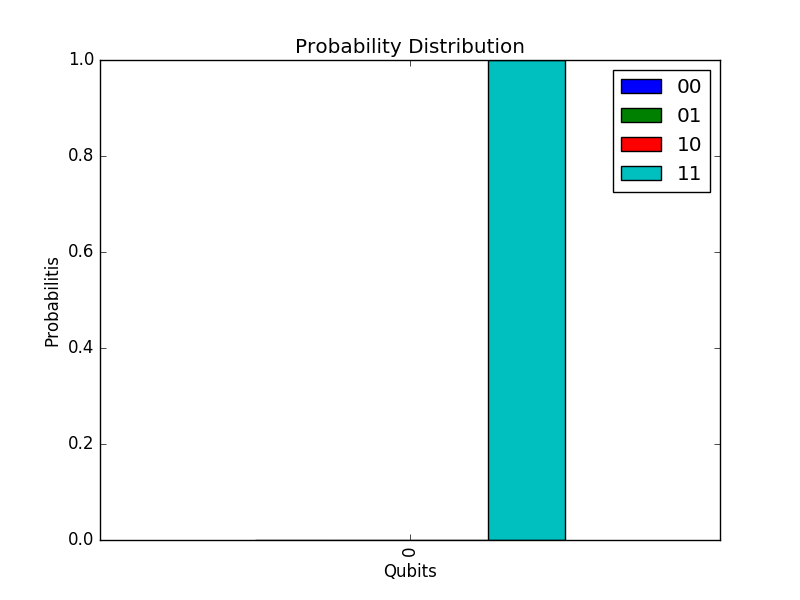
\includegraphics[scale=0.3]{A11_1}}%
\caption{Probability Distribution, without noise}
\end{figure}
\begin{thebibliography}{9}
\bibitem{knuthwebsite}
\texttt{http://www-reynal.ensea.fr/docs/iq/QC10th.pdf}
\bibitem{knuthwebsite}
\texttt{https://en.wikipedia.org/wiki/Grover's algorithm}
\bibitem{knuthwebsite}
\texttt{https://quantumexperience.ng.bluemix.net/qx/experience}
\bibitem{knuthwebsite}
\texttt{https://github.com/indrag49/Quantum-SimuPy}
\end{thebibliography}
\end{document}
